\chapter{Experiments}\label{chapter:experiments}
In this section, we evaluate the MAPG algorithm on six different Mujuco classic control tasks. We also compare the performance of our method with other popular continuous control algorithms. 

\section{Environments}

\subsection{Mujoco}
MuJoCo \cite{todorov2012mujoco} is a physics engine which provides simulations of various robotic environments involving contact dynamics. These environments range from simple pendulum on cart balancing problem to complex bipedal movement of a humanoid. The different Mujoco environments we used for our experiments are listed in Table \ref{tab:tasks}. Screenshots of different environments are given in Figure \ref{fig:envs}.

\subsection{TORCS}
The open racing car simulator (TORCS) is a 3D, multi-player car racing environment. \env{TORCS} provide an interface for agents to drive cars. It provides 29 sensors readings at each time-step of simulation, these sensor readings include car speed, angle with the road, distance from track etc. which are enough to make driving decisions. The car can be controlled using three actions, steer $\in [-1, 1]$, brake $\in [0,1]$ and accelerate $\in [0,1]$. In our experiments, we use 0.04 seconds long discrete time steps during simulation. During training, the reward was set proportional to the component of car velocity along the direction of road $v*\cos(\alpha)$, where $\alpha$ is the angle between the velocity vector and the center line of the track. This reward encourages forward motion.

\newpage 

\begin{figure}[H]
\centering
\begin{minipage}[b]{.45\textwidth}
  \centering
  \frame{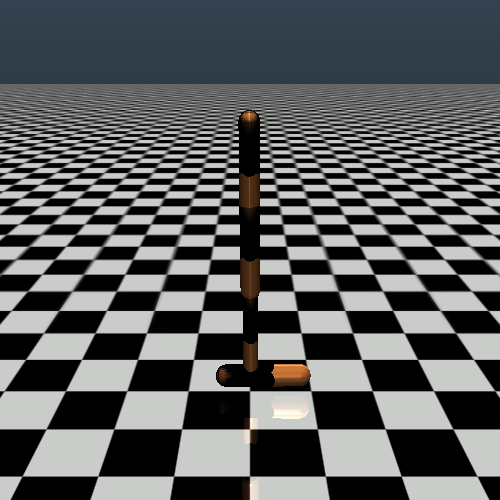
\includegraphics[width=.8\textwidth]{figures/05/hopper.png}} \\
   \env{Hopper}
   \vspace{2ex}
\end{minipage}
\begin{minipage}[b]{.45\textwidth}
  \centering
    \frame{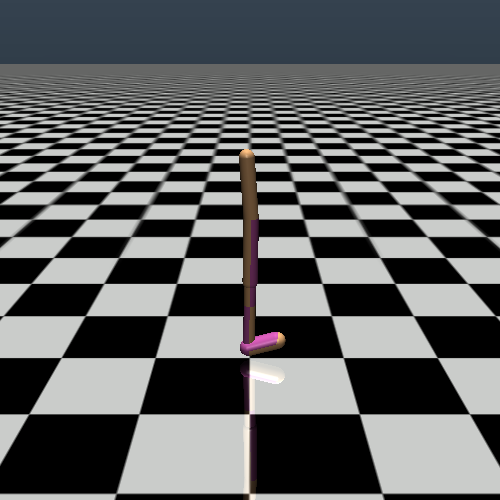
\includegraphics[width=.8\textwidth]{figures/05/walker2d.png}} \\
    \env{Walker2d}
    \vspace{2ex}
\end{minipage}
\begin{minipage}[b]{.45\textwidth}
  \centering
    \frame{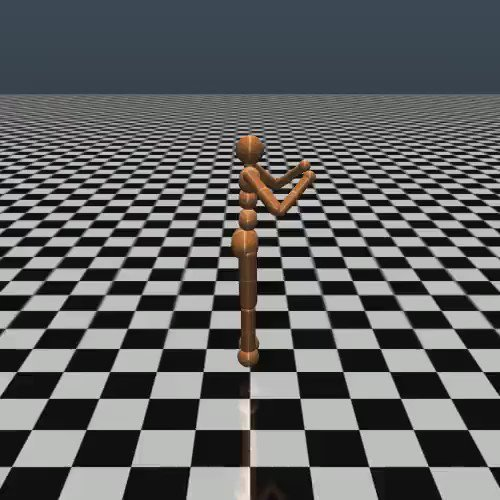
\includegraphics[width=.8\textwidth]{figures/05/humanoid.jpg}} \\
    \env{Humanoid}
    \vspace{2ex}
\end{minipage}
\begin{minipage}[b]{.45\textwidth}
  \centering
    \frame{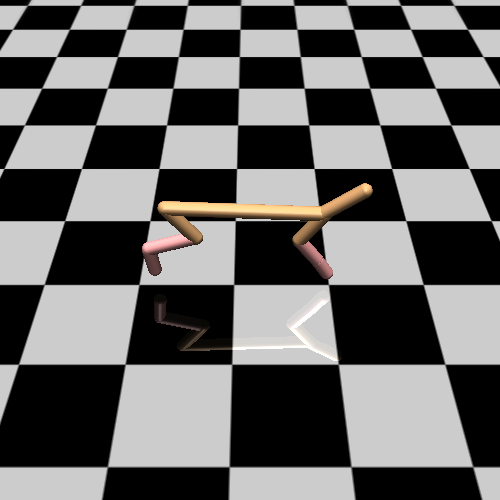
\includegraphics[width=.8\textwidth]{figures/05/halfcheetah.png}} \\
    \env{HalfCheetah}
    \vspace{2ex}
\end{minipage}
\begin{minipage}[b]{.45\textwidth}
  \centering
    \frame{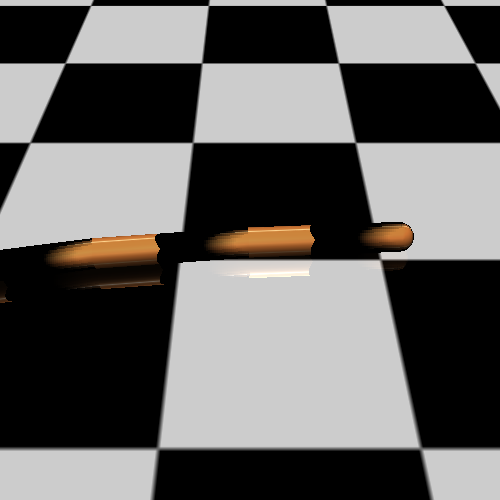
\includegraphics[width=.8\textwidth]{figures/05/swimmer.png}} \\
    \env{Swimmer}
\end{minipage}
\begin{minipage}[b]{.45\textwidth}
  \centering
    \frame{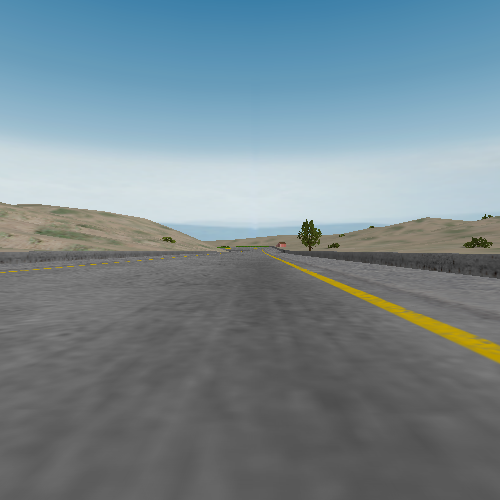
\includegraphics[width=.8\textwidth]{figures/05/torcs.png}} \\
    \env{TORCS}
\end{minipage}
  \caption{Screenshots of different environments used for evaluation.}
  \label{fig:envs}
\end{figure}


\begin{table*}[htb]
    \caption{A detailed description of the tasks used for evaluation. We have chosen a variety in tasks with continuous action space that differ in both state and action dimensionality.}
    \label{tab:tasks}
    \vskip 0.15in
    \begin{center}
        \begin{small}
            \begin{sc}
                \begin{tabular}{lrrl}
                    Task  & Action Dimension & State Dimension & Description\\
                    \hline \vspace{-0.75em} \\ 
                    \env{Pendulum} & 1 & 3 & Pendulum on a cart.\\ 
                    \env{Hopper} & 3 & 11 & One legged robot.\\ 
                    \env{Walker2d} & 6 & 17 & Two dimensional bipedal robot.\\
                    \env{Humanoid} & 17 & 376 & Three dimensional bipedal robot.\\
                    \env{HalfCheetah} & 6 & 17 & Two leg robot.\\
                    \env{Swimmer} & 2 & 6 & Three joint swimming robot.\\
                    \env{TORCS} & 3 & 29 & Control car in 3D simulation.\\ 
                \end{tabular}
            \end{sc}
        \end{small}
    \end{center}
    \vskip -0.1in
\end{table*}


\section{Training Setup}
Here we describe the setup used for training different algorithms.

\subsection{MAPG and DDPG}
We use the OpenAI Gym \cite{greg2016} and the OpenAI baselines \cite{openaibase} for evaluating our experiments. The base actor and critic network architectures are fixed in all experiments. Each network has two fully connected hidden layers with 64 units each. Each fully-connected layer is followed by a ReLU non-linearity. The actor network takes the current observed state $s_t$ as input and produces $M$ normalized actions $a^{(m)}_t \in [-1, 1]^d$ by applying $\tanh$. We then scale the predicted actions to the actual range specific to the current environment. This allows us to have the same learning rate even when dealing with different action ranges. From the $M$ actions $a^{(m)}_t$, a single action $a_t$ is randomly chosen with equal probability. 

The critic network uses the current state $s_t$ and action $a_t$ as input and outputs a scalar value ($Q$-value). The action value is concatenated with the output of the first layer followed by one hidden layer and an output layer with one unit. The critic network is trained by minimizing the mean square loss between the calculated discounted reward and the computed $Q$ value. 

The actor network is trained by computing the policy gradient from the $Q$-value of the chosen action. The network weights of the last layer are only updated for the selected action. This is achieved by setting a zero loss/gradient for the remaining $M-1$ actions. 
Ornstein-Uhlenbeck process noise is added to the action values from the actor for exploration. The parameters for the OU process are fixed for all experiments as $\mu=0$, $\sigma=0.2$ and $\theta=.15$. The training is carried out for a total of two million steps in all tasks.

\subsection{A3C}
For A3C training, we use same actor-critic networks as for the earlier experiment. The output of actor network is a mean vector ($\mu_a$) (one for each action value) and a scalar standard deviation ($\sigma^2$, shared for all actions). The actions values are sampled from the normal distribution $\mathcal{N}(\mu_a, \sigma^2)$. We used differential entropy of a normal distribution to encourage exploration with weight $10^{-4}$. The networks are trained with four asynchronous threads and the Adam optimizer is used to train the networks.

\subsection{SVG}
SVG(0) is the model-free variant of stochastic value gradients. SVG(0) is very similar to DDPG, but the policy is made stochastic by parameterizing the actor with a random variable sampled from $\mathcal{N}(0, 1)$. We used off-policy training with experience replay for training SVG(0).


\section{Results}
For more meaningful quantitative results, we report the average reward over 100 episodes with different values of $M$ for various tasks in Table \ref{tab:mujocoscore}. In Addition to the scores of MAPG, we report the scores of DDPG, A3C and SVG(0) which are the closest related methods from the literature. 
For almost all environments we score higher with $M=5$. 
The lower performance in the \env{Humanoid} task for $M=5$ might be explained by the drastically higher dimensionality of the world state in this task which makes it more difficult to observe.

The scores of policy based reinforcement learning algorithms can vary a lot depending on network hyper-parameters, reward function and codebase/framework as outlined in \cite{henderson2017deep}. To minimize the variation in score due to these factors, we fixed all parameters of different algorithms and only studied changes on the score by varying $M$. Our metric for performance in each task is average reward over 100 episodes by an agent trained for 2 million steps.
This evaluation hinders actors with high $M$ since in every training step only a single out of the $M$ actions will be updated per state. Thus, in general actors with the higher number of action proposals, will need a longer time to learn a meaningful distribution of action. This also means that an actor with higher $M$ will take longer to train all heads sufficiently long. This is partially remedied by the fact that we only split the last layer of the actor into the different actions. With this, most of the actor is updated at every training step and the additional number of training iterations scales slower than linear with increased $M$.

In Figure \ref{fig:stddev}, we studied the variance in action values for $M=10$ during training together with the achieved reward. The standard deviation of actions generated by MAPG decreases with time.
As the network converges to a good policy (increase in expected reward) the variation in action values is reduced. However, there are some spikes in standard deviation even when the network has converged to a better policy. It shows that there are situations in which the policy sees multiple good actions (with high $Q$-value) which can be exploited using MAPG.

This is an interesting aspect of the algorithm. In many tasks, there exist a good amount of states where only one single action is optimal. In these cases we expect all actions of MAPG to collapse into a single (or very similar) action. However, in certain situations, it might be beneficial to act non-deterministically. We will analyze this observation further in the next section.

In our experiments, A3C performed poorly than DDPG in all tasks and was not able to learn a good policy for \env{Humanoid} task. SVG(0) performed rather poorly on almost all tasks.

\subsection{Mujoco}
We show the box plots for the scores of Mujoco environments in Figure \ref{fig:boxplot}, where we can see that the overall score usually increases with $M$. If we set $M=1$ our algorithm is equal to DDPG, so its performance can also be seen in Figure \ref{fig:boxplot}.
\env{HalfCheetah} has the most unstable training procedure for all algorithms, often a good policy is lost and the algorithms degenerate back to a zero reward policy where they begin to learn again during training.


\subsection{TORCS}
In \env{TORCS} experiments, MAPG with $M=10$ was able to complete multiple laps of the track, whereas the DDPG based agent could not complete even one lap of the track. The average distance traveled over 100 episodes by DDPG is 807m and 5882m (both in meters) for our MAPG agent.

\begin{figure}[hH]
    \centering
    \begin{minipage}[b]{.45\textwidth}
        \centering
        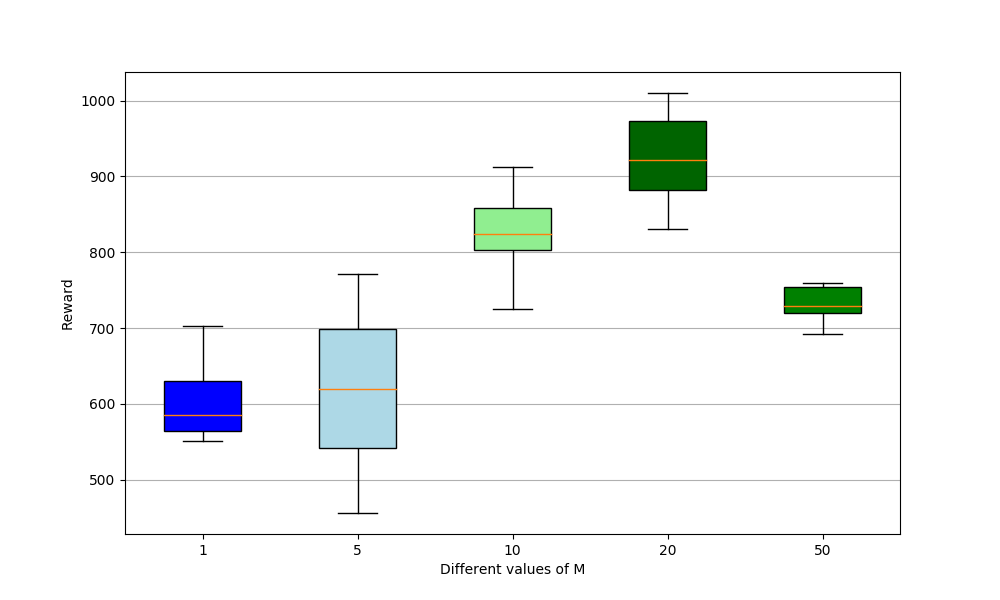
\includegraphics[width=0.95\textwidth]{figures/box_plot.png} \\
        (a) \env{Hopper}.
        \label{fig:boxplot:hopper}
    \end{minipage}
    \begin{minipage}[b]{.45\textwidth}
        \centering
        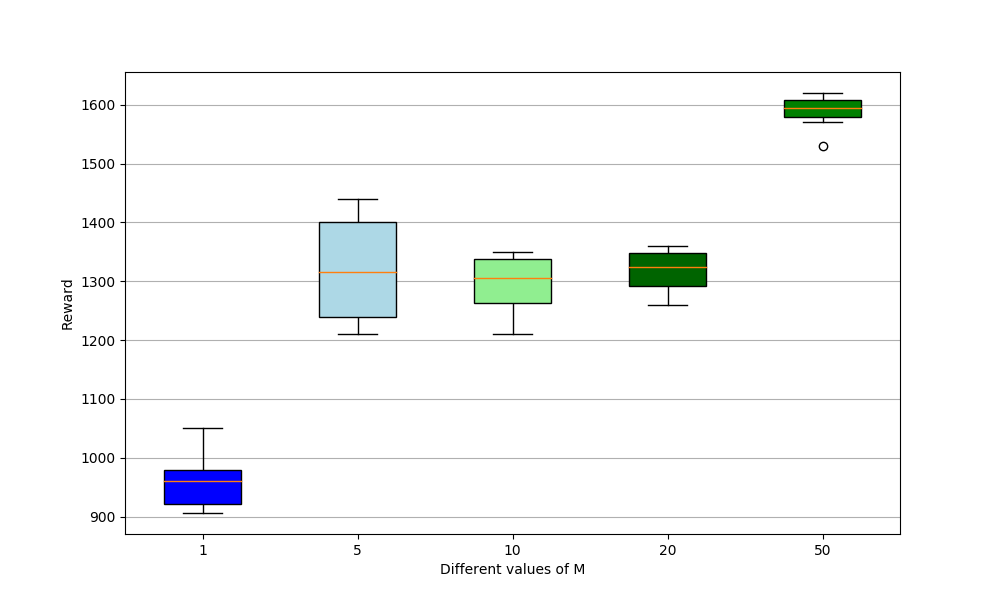
\includegraphics[width=0.95\textwidth]{figures/walker2d_box_plot.png} \\
        (b) \env{Walker2d}.
        \label{fig:boxplot:walker}
    \end{minipage}
    \begin{minipage}[b]{0.45\textwidth}
        \centering
        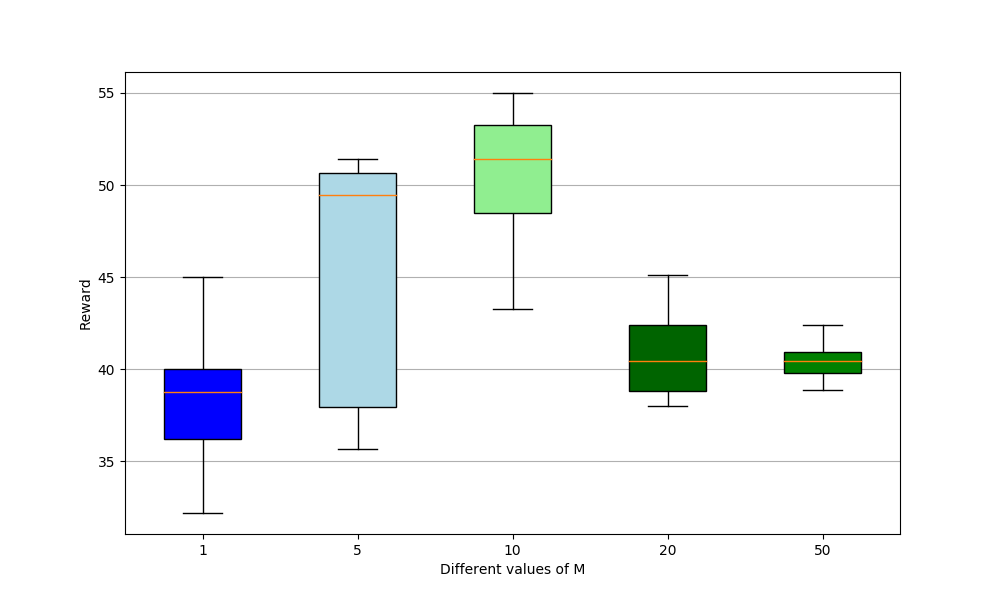
\includegraphics[width=0.95\textwidth]{figures/Swimmer-v1.png} \\
        (c) \env{Swimmer}.
    \end{minipage}
    \begin{minipage}[b]{0.45\textwidth}
        \centering
        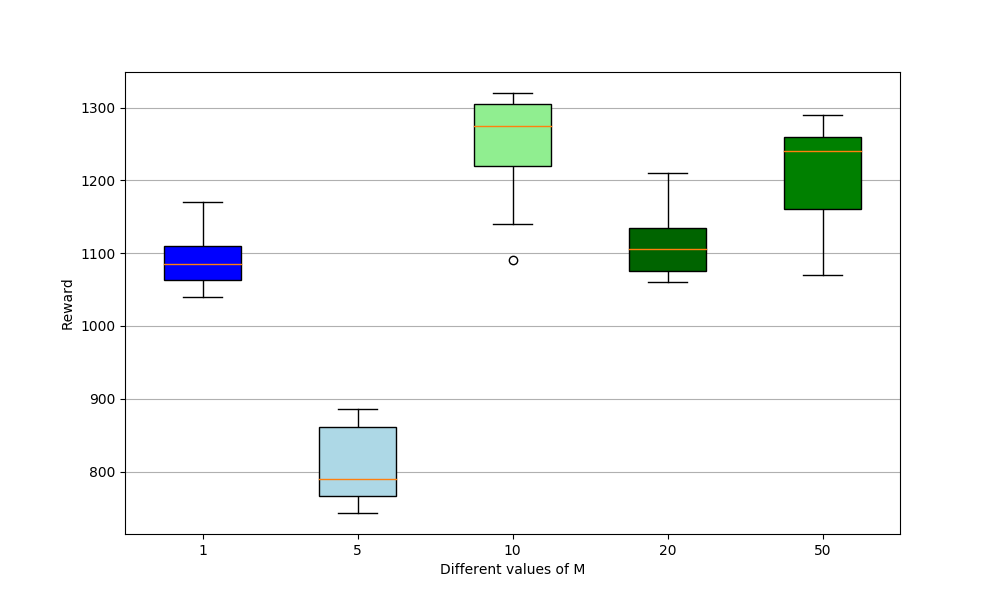
\includegraphics[width=0.95\textwidth]{figures/Humanoid-v1.png} \\
        (d) \env{Humanoid}.
    \end{minipage}
    
    \begin{minipage}[b]{0.45\textwidth}
        \centering
        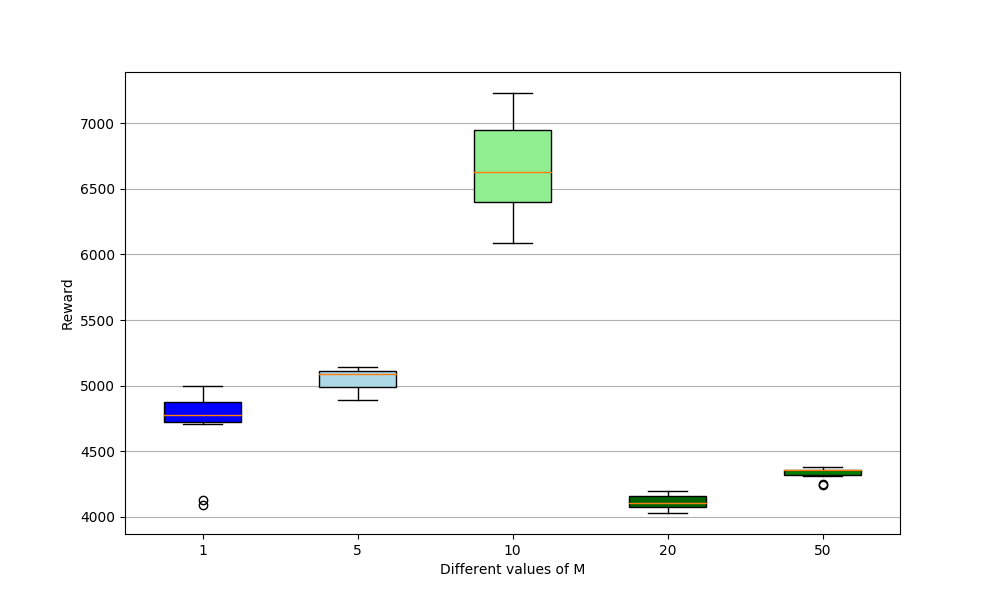
\includegraphics[width=0.95\textwidth]{figures/HalfCheetah-v1.png} \\
        (e) \env{HalfCheetah}.
     \end{minipage}
    \caption{Variation in score of (from top left) \env{Hopper}, \env{Walker2d}, \env{Swimmer}, \env{Humanoid} and \env{HalfCheetah} with different values of $M$.}
    \label{fig:boxplot}
    % \caption{Variation in score of Hopper and Walker2d with different values of $M$.}
\end{figure}


\begin{table}[htb]
    \caption{Comparison of average score $\pm 3\sigma$ over 100 episodes for Mujoco tasks between DDPG and MAPG.}
    \label{tab:mujocoscore}
    \vskip 0.15in
    \begin{center}
        \begin{small}
            \begin{sc}
                \begin{tabular}{l|rrrrr}
                    Environment & DDPG & $M=5$ & $M=10$ & $M=20$ & $M=50$\\
                    \hline \vspace{-0.75em} \\ 
                    \env{Hopper-v1}        & 603 $\pm$ 76  & 619  $\pm$ 157 &  824          $\pm$ 94    &\textbf{923} $\pm$ 90 & 732 $\pm$  34 \\
                    \env{Walker2d-v1}   & 960 $\pm$ 72  & 1318 $\pm$ 115 & 1297          $\pm$ 70    & 1319 $\pm$  50       &\textbf{1589} $\pm$  45 \\
                    \env{Humanoid-v1}   &1091 $\pm$ 65  & 809  $\pm$ 72  & \textbf{1248} $\pm$ 115  & 1112 $\pm$ 75           & 1212 $\pm$ 110 \\
                    \env{HalfCheetah-v1}&4687 $\pm$ 455 & 5052 $\pm$ 125 & \textbf{6659} $\pm$ 570    & 4116 $\pm$ 85        & 4333 $\pm$ 70 \\
                    \env{Swimmer-v1}    &  38 $\pm$ 7   & 45   $\pm$ 8   & \textbf{51}   $\pm$  6    &  41 $\pm$   4        &  40 $\pm$   2 \\    
                \end{tabular}
            \end{sc}
        \end{small}
    \end{center}
    \vskip -0.1in
\end{table}


\begin{table}[htb]
    \caption{Comparison of average score $\pm 3\sigma$ over 100 episodes for Mujoco tasks between DDPG, A3C, SVG(0) and MAPG with $M=10$.}
    \label{tab:score_svg}
    \vskip 0.15in
    \begin{center}
        \begin{small}
            \begin{sc}
                \begin{tabular}{l|rrrr}
                    Environment & DDPG & A3C & SVG(0) & $M=10$ \\
                    \hline \vspace{-0.75em} \\ 
                    \env{Hopper-v1}        & 603 $\pm$ 76 & 532 $\pm$ 105    & 181 $\pm$ 62 &  \textbf{824} $\pm$ 94 \\
                    \env{Walker2d-v1}        & 960 $\pm$  72 & 764 $\pm$ 112 & 613 $\pm$ 118    & \textbf{1297} $\pm$ 70    \\
                    \env{Humanoid-v1}        &1091 $\pm$ 65 & 281 $\pm$ 40 & 412 $\pm$ 82 &\textbf{1248} $\pm$  115 \\
                    \env{HalfCheetah-v1}    &4687 $\pm$ 455 & 3803 $\pm$ 125 & 429 $\pm$ 76 &\textbf{6659} $\pm$ 570 \\
                    \env{Swimmer-v1}        &  38 $\pm$   7 &  33 $\pm$ 10 & 41 $\pm$ 5 &\textbf{51} $\pm$   6    \\
                \end{tabular}
            \end{sc}
        \end{small}
    \end{center}
    \vskip -0.1in
\end{table}

\section{Action Variance Analysis}
\begin{figure}[H]
    \centering
    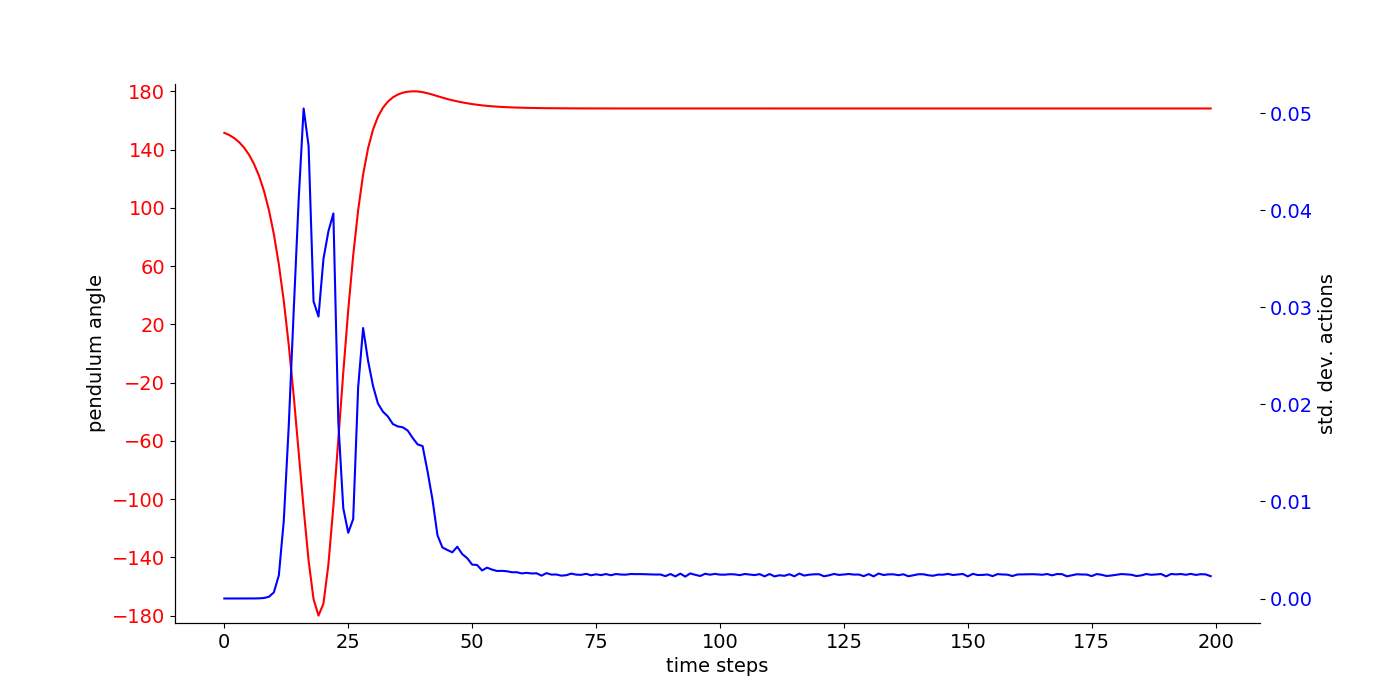
\includegraphics[width=.9\linewidth]{figures/pendulum_angle_variance.png}
    \caption{Standard deviation and angle during one episode of the \env{Pendulum} environment. An angle of $\pm180$ is the target inverted pose. $0$ is hanging downwards.}
    \label{fig:devangle}
\end{figure}

We use the simple \env{Pendulum} environment to analyze the variance during one episode. The task is the typical inverted pendulum task, where a cart has to be moved such that it balances a pendulum in an inverted position.

Figure \ref{fig:devangle} plots standard deviation and the angle of the pendulum. Some interesting relationships can be observed. The variance exhibits two strong spikes that coincide with an angle of $0$ degrees. This indicates that the agent has learned that there are two ways it can swing up the pole: either by swinging it clockwise or counterclockwise. A deterministic agent would need to pick one over the other instead of deciding randomly. Further, once the target inverted pose (at 180 degrees) is reached the variance does not go down to 0. This means that for the agent a slight jitter seems to be the best way to keep the pendulum from gaining momentum in one or the other direction.

Further, it seems to have learned that slowing the pendulum down close to the upright position, is possible with some noisy torque which explains the second peak in Figure \ref{fig:devangle} at timesteps 30-40. 

With this analysis, we could show that a MAPG agent can learn meaningful policies. The variance over predicted actions can give additional insight into the learned policy and results in a more diverse agent that can, for example, swing up the pole in two different directions instead of picking one.

\begin{figure}[H]
\centering
\begin{minipage}[b]{.9\textwidth}
  \centering
  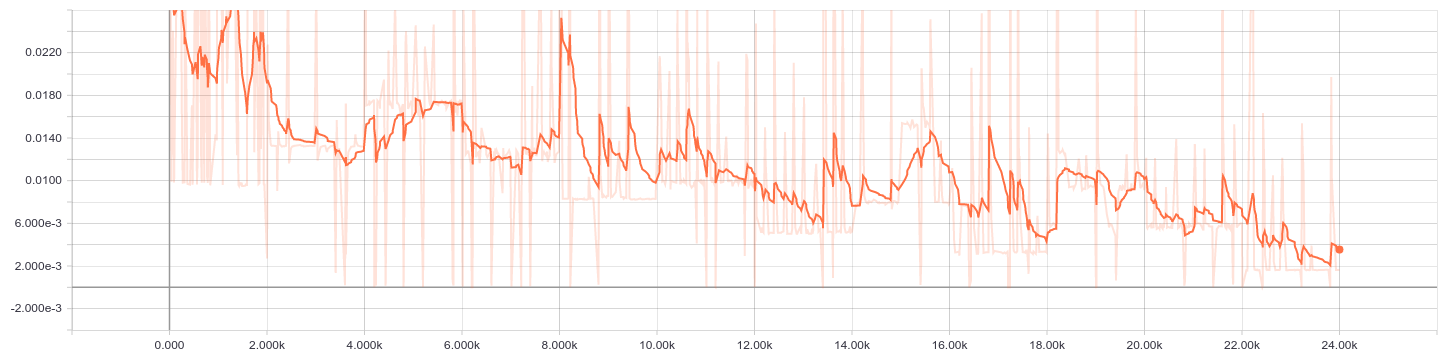
\includegraphics[width=\textwidth]{figures/std_eval.png} \\
  (a) Standard deviation in action values.
\end{minipage}

\begin{minipage}[b]{.9\textwidth}
  \centering
    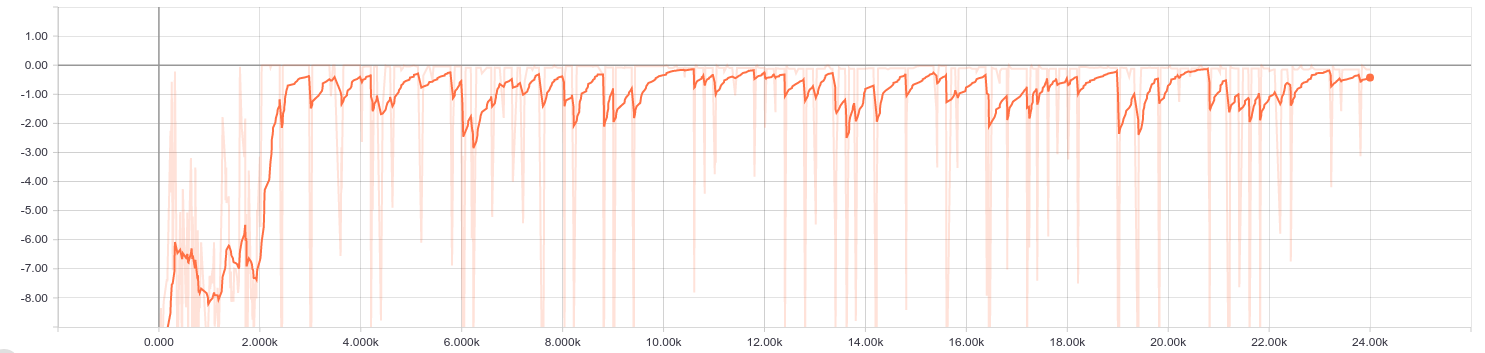
\includegraphics[width=\textwidth]{figures/reward_eval.png} \\
   (b) Reward.
\end{minipage}
  \caption{Standard deviation and reward with $M=10$ for the \env{Pendulum} task during training.}
  \label{fig:stddev}
\end{figure}


\section{Value Variance Analysis}
To validate the proof that an optimal policy consists of $M$ actions with equal value at each timestep we compute the average relative deviation from the mean action value as
\begin{equation}
\frac{\max_m Q^\rho(s_{t},\rho_m(s_{t})) - \min_m Q^\rho(s_{t},\rho_m(s_{t}))}{\frac{1}{m}\sum_m{| Q^\rho(s_{t},\rho_m(s_{t})) |}}.
\end{equation}
This estimates how much the maximal difference between $Q$ values fluctuates in percent over an episode. For the \env{Pendulum} environment with $M=10$ we compute an average, relative deviation of $0.2\%$. This means that indeed the predicted value for all actions is very close to equal. 

We have further evaluated different strategies for choosing an action during evaluation of a policy. Even though values are very close we have tried choosing the highest value action instead of uniform random choice and observed identical performance. Further, also selecting a fixed action - for example always the first action - did not change the performance of the method. This further validates that the predicted actions are indeed equal in performance as expected from our proof in Section \ref{03:mapg_proof}.

\section{Effect on Exploration}

Here, we study the effect of MAPG on exploration during training. We compare the performance of DDPG and MAPG during training with and without any external noise on \env{Pendulum}, \env{HalfCheetah} and \env{Walker2d} environments. Figure \ref{fig:exploration-hc} shows the average reward during training with DDPG and MAPG $M=10$. The policy trained using MAPG converges to better average reward than DDPG in all cases. Moreover, the performance of MAPG without any external exploration is comparable to DDPG with added exploration noise. This means MAPG can explore the state space enough to find a good policy.

In the \env{HalfCheetah} environment we can see that using exploration creates a much bigger performance difference between DDPG and MAPG than without. The difference sets in after about 500 epochs. This is an indication that in the beginning of training the actions predicted by MAPG are similar to the one from DDPG. The noise later helps to pull the $M$ actions apart, leading to a more diverse policy with better reward. In \env{Walker2d} environment, the difference in performance with MAPG and DDPG is not wide as \env{HalfCheetah}. This could be because $M=10$ is not optimal for this environment.

Similar to our other experiments we find that MAPG agents explore more possibilities due to their stochastic nature and can then learn more stable and better policies. 


\begin{figure*}[h]
    \centering
    \begin{minipage}[b]{.8\textwidth}
        \centering
        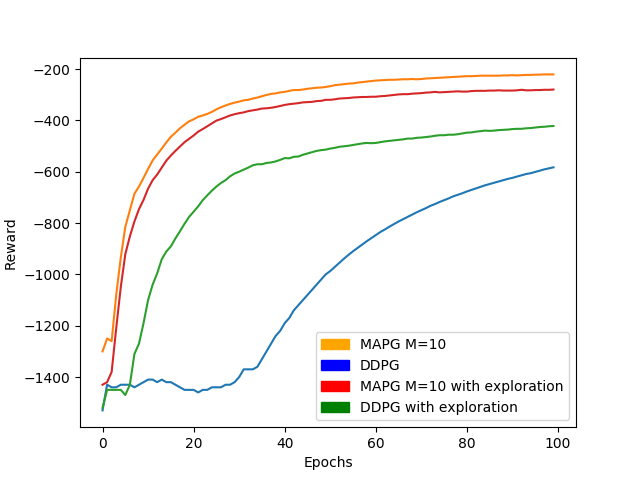
\includegraphics[width=.9\textwidth]{figures/pendulum_expl.png} \\
        (a) \env{Pendulum}.
    \end{minipage}
    \quad
    \begin{minipage}[b]{.8\textwidth}
        \centering
        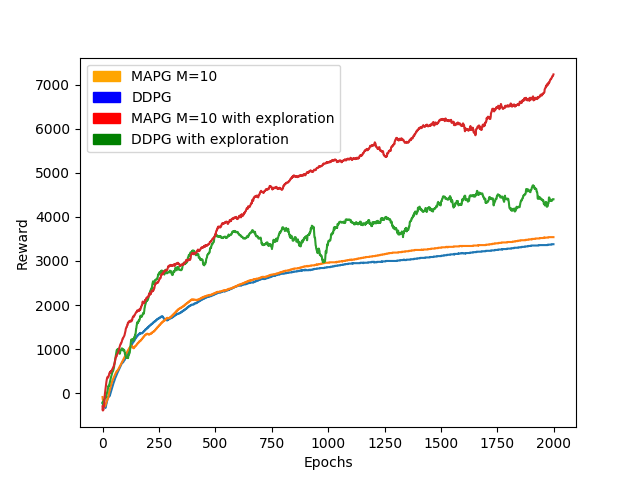
\includegraphics[width=.9\textwidth]{figures/halfcheetah_expl.png} \\
        (b) \env{HalfCheetah}.
    \end{minipage}
    \caption{Performance curves for two environments with and without external exploration noise on DDPG and MAPG: original DDPG with OU process noise (green), DDPG without any exploration noise (blue), MAPG (M=10) with OU process noise (red) and MAPG (M=10) without OU process noise (orange).}
    \label{fig:exploration-hc}
\end{figure*}

\begin{figure*}[h]
\centering
    \begin{minipage}[b]{.8\textwidth}
        \centering
        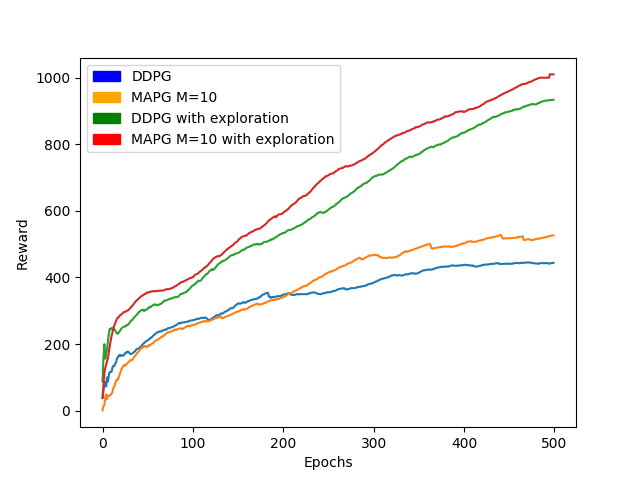
\includegraphics[width=.9\textwidth]{figures/walker_expl.png}
    \end{minipage}
    \caption{Performance of \env{Walker2d} on DDPG and MAPG with and without external noise.}
    \label{fig:exploration-walker}
\end{figure*}
